\section*{2025年普通高等学校招生全国统一考试(新高考2卷)}


使用地区：海南、辽宁、重庆、吉林、黑龙江、贵州、广西、甘肃、云南、四川、陕西、山西、内蒙古、青海、宁夏\\

\begin{frame}[allowframebreaks]{第1题}
\begin{frame}[allowframebreaks]{第1题}
\begin{example}
样本数据2，8，14，16，20的平均数为\blankbox
\begin{choices}
\choice{$8$}
\choice{$9$}
\choice{$12$}
\choice{$18$}
\end{choices}
\end{example}
\end{frame}

\begin{answer}
C
\end{answer}
\begin{solutions}
平均数计算公式：$\bar{x}=\dfrac{2+8+14+16+20}{5}=12$，故选C。
\end{solutions}
\end{frame}
t{i}$，则$\dfrac{1}{z-1}=$\blankbox
\begin{choices}
\choice{$-\text{i}$}
\choice{$\text{i}$}
\choice{$-1$}
\choice{$1$}
\end{choices}
\begin{proof}
	\begin{answer}
		A
	\end{answer}
	\begin{solutions}
		由$z=1+\text{i}$，得$z-1=\text{i}$，则$\dfrac{1}{z-1}=\dfrac{1}{\text{i}}=-\text{i}$，故选A。
	\end{solutions}
\end{proof}
\end{example}

\begin{frame}[allowframebreaks]{第3题}
\begin{frame}[allowframebreaks]{第3题}
\begin{example}
设集合$A=\{-4,0,1,2,8\}$，$B=\{x\mid x^3=x\}$，则$A\cap B=$\blankbox
\begin{choices}
\choice{$\{0,1,2\}$}
\choice{$\{1,2,8\}$}
\choice{$\{2,8\}$}
\choice{$\{0,1\}$}
\end{choices}
\end{example}
\end{frame}

\begin{answer}
D
\end{answer}
\begin{solutions}
由$x^3=x$得$x(x^2-1)=0$，解得$x=-1,0,1$，即$B=\{-1,0,1\}$。
		又$A=\{-4,0,1,2,8\}$，故$A\cap B=\{0,1\}$，选D。
\end{solutions}
\end{frame}
考][第7题]
记$S_n$等差数列$\{a_n\}$的前$n$项和，若$S_3=6$，$S_5=-5$，则$S_6=$\blankbox
\begin{choices}
\choice{$-20$}
\choice{$-15$}
\choice{$-10$}
\choice{$-5$}
\end{choices}
\end{example}

\begin{frame}[allowframebreaks]{第8题}
\begin{frame}[allowframebreaks]{第8题}
\begin{example}
设$0<\theta<\pi$，若$\cos\dfrac{\theta}{2}=\dfrac{\sqrt{5}}{5}$，则$\sin\left(\theta-\dfrac{\pi}{4}\right)=$\blankbox
\begin{choices}
\choice{$\dfrac{\sqrt{2}}{10}$}
\choice{$\dfrac{\sqrt{2}}{5}$}
\choice{$\dfrac{3\sqrt{2}}{10}$}
\choice{$\dfrac{7\sqrt{2}}{10}$}
\end{choices}
\end{example}
\end{frame}

\end{frame}
l AD$，$AB=3AD$，$CD=2AD$．将四边形$EFDA$沿$EF$翻折至四边形$EFD'A'$，使得面$EFD'A'$与面$EFCB$所成的二面角为$60^\circ$．
\begin{enumerate}
    \item 证明：$A'B\parallel$平面$CD'F$；
    \item 求平面$BCD'$与面$EFD'A'$所成二面角的正弦值．
\end{enumerate}

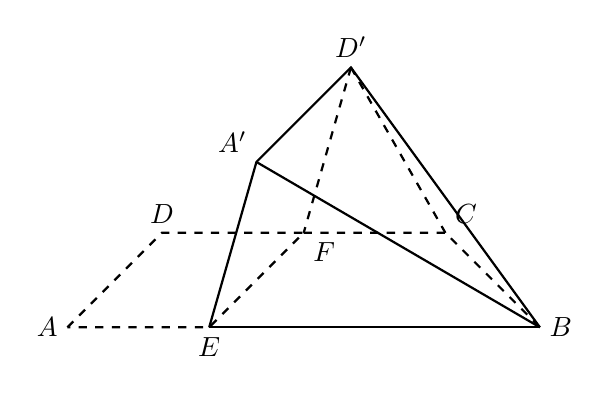
\begin{tikzpicture}[scale=1.5, >=latex]
	% 1. 定义底面固定坐标（不变）
	\coordinate (A) at (-1.5,-0.5);
	\coordinate (D) at (-0.7,0.3);
	\coordinate (E) at (-0.3,-0.5);
	\coordinate (F) at (0.5,0.3);
	
	% 右侧固定点（不变）
	\coordinate (B) at (2.5,-0.5);
	\coordinate (C) at (1.7,0.3);
	
	% 核心修改：调整 A'、D' 坐标，模拟 120° 空间翻折角
	\coordinate (A') at (0.1, 0.9);   % 120°翻折后 A 的投影
	\coordinate (D') at (0.9, 1.7);   % 120°翻折后 D 的投影
	
	% 2. 绘制不可见线与原平面残留（虚线段）
	\draw[dashed, thick] (A) -- (D) -- (F) -- (E) -- (A);
	\draw[dashed, thick] (F) -- (C) -- (B);
	\draw[dashed, thick] (D') -- (F);
	\draw[dashed, thick] (D') -- (C);
	
	% 3. 绘制可见线（实线段）
	\draw[thick] (E) -- (B);
	\draw[thick] (E) -- (A') -- (D') -- (B);
	\draw[thick] (A') -- (B);
	
	% 4. 顶点标注
	\node[left] at (A) {$A$};
	\node[above] at (D) {$D$};
	\node[below] at (E) {$E$};
	\node[below right] at (F) {$F$};
	\node[right] at (B) {$B$};
	\node[above right] at (C) {$C$};
	\node[above left] at (A') {$A'$};
	\node[above] at (D') {$D'$};
	
\end{tikzpicture}
\end{example}

\begin{frame}[allowframebreaks]{第18题}
\begin{frame}[allowframebreaks]{第18题}
\begin{example}
已知函数$f(x)=\ln(1+x)-x+\dfrac{1}{2}x^2-kx^3$，其中$0<k<\dfrac{1}{3}$．
\begin{enumerate}
    \item 证明：$f(x)$在$(0,+\infty)$存在唯一极值点和唯一零点；
    \item 设$x_1,x_2$为$f(x)$在$(0,+\infty)$的极值点和零点．
    \begin{enumerate}
        \item 设函数$g(t)=f(x_1+t)-f(x_1-t)$，证明：$g(t)$在$(0,x_1)$单调递减；
        \item 比较$2x_1$与$x_2$的大小，并证明．
    \end{enumerate}
\end{enumerate}
\end{example}
\end{frame}

\end{frame}
